\documentclass[tikz,border=3pt]{standalone}
\usepackage[T1]{fontenc}
\usepackage[default]{sourcesanspro}
\usepackage{fontawesome5}
\usepackage{xcolor}
\usepackage{tikz}
\usetikzlibrary{arrows.meta,positioning,fit,backgrounds,calc}

\definecolor{ink}{HTML}{1C2430}
\definecolor{blue}{HTML}{1B4F72}
\definecolor{band}{HTML}{F4F7FB}
\definecolor{chipbg}{HTML}{E6EEF5}
\definecolor{amber}{HTML}{9A3412}
\definecolor{amberbg}{HTML}{FDE8D8}
\definecolor{mut}{HTML}{4A5562}
\definecolor{line}{HTML}{1C2430}
\definecolor{optbg}{HTML}{F7F8F9}
\definecolor{passbg}{HTML}{1B4F72}
\definecolor{unkbg}{HTML}{ECEFF1}

\setlength{\fboxsep}{1.15pt}
\setlength{\fboxrule}{0pt}
\newcommand{\chip}[1]{\colorbox{chipbg}{\textcolor{ink}{\scriptsize #1}}\hspace{0.18em}}
\newcommand{\ochip}[1]{\colorbox{amberbg}{\textcolor{amber}{\scriptsize #1}}\hspace{0.18em}}
\newcommand{\pchip}[1]{\colorbox{passbg}{\textcolor{white}{\scriptsize #1}}\hspace{0.18em}}
\newcommand{\uchip}[1]{\colorbox{unkbg}{\textcolor{mut}{\scriptsize #1}}\hspace{0.18em}}
\newcommand{\hd}[2]{{\small #1\,\textbf{#2}}}
\newcommand{\gl}[1]{{\scriptsize\color{mut}#1}}

\newsavebox{\neticon}
\sbox{\neticon}{%
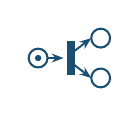
\begin{tikzpicture}[x=1pt,y=1pt,line cap=round,line join=round,baseline=-3pt]
  \draw[blue,line width=0.75pt] (0,0) circle (3.4);
  \fill[blue] (0,0) circle (1.15);
  \draw[blue,line width=0.7pt,-{Stealth[length=1.5mm]}] (3.5,0) -- (9.2,0);
  \fill[blue] (10.6,-6.2) rectangle (13.2,6.2);
  \draw[blue,line width=0.7pt,-{Stealth[length=1.5mm]}] (13.2,2.6) -- (19.2,7.2);
  \draw[blue,line width=0.7pt,-{Stealth[length=1.5mm]}] (13.2,-2.6) -- (19.2,-7.2);
  \draw[blue,line width=0.75pt] (22.6,7.2) circle (3.4);
  \draw[blue,line width=0.75pt] (22.6,-7.2) circle (3.4);
\end{tikzpicture}}

\begin{document}
\begin{tikzpicture}[
  font=\sffamily,
  x=1cm,y=1cm,
  line cap=round,line join=round,
  card/.style={draw=ink,fill=white,rounded corners=1.2pt,line width=0.55pt,
               align=left,inner sep=5.5pt,text=ink},
  our/.style={card,draw=blue,line width=0.7pt},
  ext/.style={card,draw=black!45,line width=0.5pt},
  arr/.style={-{Stealth[length=2.05mm,width=1.55mm]},line width=0.65pt,draw=ink},
  arrb/.style={arr,draw=blue},
  fb/.style={-{Stealth[length=2.05mm,width=1.55mm]},line width=0.7pt,draw=amber,
             dashed,dash pattern=on 2.4pt off 1.5pt},
  lab/.style={font=\sffamily\scriptsize,fill=white,inner sep=1.3pt,text=ink},
  ph/.style={font=\sffamily\bfseries\scriptsize,text=blue,inner sep=0pt}
]

% ---------- 1 Propose ----------
\node[card,anchor=north west,text width=4.05cm] (req) at (0,0) {%
  \hd{\faIcon{file-alt}}{Requirements}\\[1pt]
  \gl{natural language}\\[3pt]
  \chip{task text}\chip{terminal line}\\[3pt]
  \gl{The frozen contract is not in the prompt. It is read only by the Petri explorer.}%
};

\node[card,anchor=north west,text width=3.15cm] (llm) at (4.85,0) {%
  \hd{\faIcon{project-diagram}}{LLM}\\[1pt]
  \gl{proposes a skeleton}\\[3pt]
  \gl{given}\\[1pt]
  \chip{requirements}\\[2pt]
  \chip{DSL grammar}\\[2pt]
  \chip{last counterexample}\\[3pt]
  \gl{not given: contract goals}%
};

\node[our,anchor=north west,text width=7.55cm] (skel) at (8.75,0) {%
  \hd{\faIcon{code}}{Skel}\hfill\gl{skeleton DSL}\\[2pt]
  \chip{mutex}\chip{condvar}\chip{semaphore}\chip{channel}\chip{atomic}\\[2pt]
  \chip{lock}\chip{spawn}\chip{scope}\chip{compute}\\[3pt]
  \colorbox{black!4}{\ttfamily\scriptsize
    fn t1() \{\, lock a \{\, lock b \{\, compute "update";\,\}\,\}\,\}}\\[2pt]
  \gl{Checks and counterexamples are mapped back onto these lines.}%
};

\draw[arr] (req.east) -- (llm.west) node[lab,midway] {prompt};
\draw[arrb] (llm.east) -- (skel.west) node[lab,midway,text=blue] {.skel};

% ---------- 2 Check ----------
\path let \p1=(req.south), \p2=(llm.south), \p3=(skel.south) in
  coordinate (row1s) at (0,{min(\y1,\y2,\y3)});
\node[our,anchor=north west,text width=6.35cm] (cir) at ($(row1s)+(0,-0.78)$) {%
  \hd{\faIcon{layer-group}}{ConcIR}\hfill\gl{sole semantics}\\[2pt]
  \gl{Lowering is total: a checked skeleton becomes ConcIR plus a source map. The DSL adds no meaning.}\\[3pt]
  \chip{validate}\chip{support}\chip{source map}\\[3pt]
  \gl{ops}\\[1pt]
  \chip{lock / unlock}\chip{send / recv}\\[2pt]
  \chip{wait / notify}\chip{acquire / release}%
};

\node[our,anchor=north west,text width=9.15cm,fill=band] (petri) at ($(row1s)+(7.15,-0.78)$) {%
  \raisebox{-0.15em}{\usebox{\neticon}}\hspace{0.35em}\textbf{Petri exploration}\hfill\gl{bounded schedules}\\[2pt]
  {\scriptsize
  \begin{tabular}{@{}l@{\hspace{1.15em}}l@{}}
    \textbf{Unmet requirements} & \textbf{Concurrency bugs}\\
    goal not reached & deadlock\\
    preserved behaviour missed & lock-order cycle\\
    & lost wakeup\\
    & atomicity violation\\
  \end{tabular}}\\[3pt]
  \pchip{PASS}\ochip{counterexample}\uchip{UNKNOWN $\neq$ safe}%
};

\draw[arrb] (cir.east) -- (petri.west) node[lab,midway,text=blue] {encode};

% ---------- 3 Realize ----------
\path let \p1=(cir.south), \p2=(petri.south) in
  coordinate (row2s) at (0,{min(\y1,\y2)});
\node[card,anchor=north west,text width=5.55cm] (rust) at ($(row2s)+(0,-0.78)$) {%
  \hd{\faIcon{cube}}{Rust}\hfill\gl{concrete program}\\[2pt]
  \gl{On PASS, the LLM writes Rust from the accepted skeleton and the requirements.}\\[3pt]
  \chip{verified Skel}\chip{requirements}\\[2pt]
  \chip{runtime concir\_sync}%
};

\node[ext,anchor=north west,text width=4.85cm] (mem) at ($(row2s)+(6.35,-0.78)$) {%
  \hd{\faIcon{shield-alt}}{Memory safety}\\[1pt]
  \gl{Rust compiler}\\[3pt]
  \chip{ownership}\\[2pt]
  \chip{borrows}\chip{lifetimes}\\[2pt]
  \gl{Safe Rust has no unchecked data races.}%
};

\node[our,anchor=north west,text width=4.85cm] (con) at ($(row2s)+(11.85,-0.78)$) {%
  \hd{\faIcon{random}}{Concurrency safety}\\[1pt]
  \gl{same Petri net}\\[3pt]
  \chip{deadlock}\\[2pt]
  \chip{lock order}\chip{wakeup}\\[2pt]
  \gl{Passed requirements bind the Rust code.}%
};

\draw[arr] (rust.east) -- (mem.west);
\draw[arrb] (mem.east) -- (con.west);

% ---------- 4 Optional ----------
\path let \p1=(rust.south), \p2=(mem.south), \p3=(con.south) in
  coordinate (row3s) at (0,{min(\y1,\y2,\y3)});
\node[ext,anchor=north west,text width=5.15cm,dashed] (ins) at ($(row3s)+(0,-0.72)$) {%
  \hd{\faIcon{search}}{Instrumentation}\\[1pt]
  \gl{while generating Skel}\\[3pt]
  \gl{Probes ride along the skeleton so a run can be checked, not only the bounded net.}\\[2pt]
  \chip{runtime trace}\chip{schedule}%
};

\node[ext,anchor=north west,text width=5.15cm,dashed] (str) at ($(row3s)+(5.85,-0.72)$) {%
  \hd{\faIcon{exchange-alt}}{Structural check}\\[1pt]
  \gl{after Rust is emitted}\\[3pt]
  \gl{The program is mapped back to a Petri net and compared with the verified one.}\\[2pt]
  \chip{same locks}\chip{same spawn}%
};

\node[ext,anchor=north west,text width=5.15cm,dashed] (tools) at ($(row3s)+(11.7,-0.72)$) {%
  \hd{\faIcon{lock}}{Generation accuracy}\\[2pt]
  {\scriptsize\faIcon{random}}\ \textbf{loom}\ \gl{interleavings}\\[1pt]
  {\scriptsize\faIcon{bug}}\ \textbf{miri}\ \gl{undefined behavior}\\[1pt]
  {\scriptsize\faIcon{lock}}\ \textbf{lockbud}\ \gl{double-lock, order}%
};

% ---------- phase bands ----------
\begin{scope}[on background layer]
  \node[ph,anchor=south west] (h1) at ($(req.north west)+(-0.05,0.16)$) {1\quad Propose};
  \node[ph,anchor=south west] (h2) at ($(cir.north west)+(-0.05,0.16)$) {2\quad Check};
  \node[ph,anchor=south west] (h3) at ($(rust.north west)+(-0.05,0.16)$) {3\quad Realize};
  \node[ph,anchor=south west] (h4) at ($(ins.north west)+(-0.05,0.16)$) {4\quad Optional};
  \node[draw=black!18,fill=black!2.5,rounded corners=1.6pt,inner sep=3.2pt,
        fit=(h1)(req)(llm)(skel)] (b1) {};
  \node[draw=blue!35,fill=blue!5,rounded corners=1.6pt,inner sep=3.2pt,
        fit=(h2)(cir)(petri)] (b2) {};
  \node[draw=black!18,fill=black!2.5,rounded corners=1.6pt,inner sep=3.2pt,
        fit=(h3)(rust)(mem)(con)] (b3) {};
  \node[draw=black!35,dashed,dash pattern=on 2pt off 1.4pt,fill=optbg,
        rounded corners=1.6pt,inner sep=3.2pt,fit=(h4)(ins)(str)(tools)] (b4) {};
\end{scope}

% gutters and the counterexample rail sit outside the cards
\coordinate (g1) at ($(b1.south)!0.52!(b2.north)$);
\coordinate (g2) at ($(b2.south)!0.52!(b3.north)$);
\draw[arrb] (skel.south) -- (skel.south |- g1) -- (cir.north |- g1) -- (cir.north)
  node[pos=0.55, above=1pt, lab, text=blue] {lower $+$ source map};
\draw[arr] (petri.south) -- (petri.south |- g2) -- (rust.north |- g2) -- (rust.north)
  node[pos=0.55, above=1pt, lab] {PASS $\cdot$ LLM writes Rust};

\node[fit=(b1)(b2)(b3)(b4), inner sep=0pt] (alls) {};
\coordinate (toprail) at ($(alls.north)+(0,0.28)$);
\coordinate (rightrail) at ($(alls.east)+(0.42,0)$);
\draw[fb] (petri.east) -- (petri.east -| rightrail)
  -- (rightrail |- toprail)
  -- (llm.north |- toprail)
  node[midway, above=1pt, font=\sffamily\scriptsize, text=amber, fill=white, inner sep=1.2pt]
  {counterexample, remapped to the Skel line; contract hidden}
  -- (llm.north);

\end{tikzpicture}
\end{document}
